\documentclass[11pt]{article}
\usepackage[a4paper,top=1.5cm,bottom=3.0cm,left=1.9cm,right=1.9cm,footskip=2.0cm]{geometry}
\usepackage{graphicx}
\usepackage[table]{xcolor}
\usepackage{ragged2e}
\usepackage{fancyhdr}
\usepackage{fontspec}
\setmainfont{Noto Sans Devanagari}
\setsansfont{Noto Sans Devanagari}
\newfontfamily\latinfont{Carlito}
\renewcommand{\familydefault}{\sfdefault}
\definecolor{titleblue}{HTML}{0F2F4A}
\definecolor{textblack}{HTML}{1A1A1A}
\definecolor{rule}{HTML}{C9C4C0}
\definecolor{muted}{HTML}{6B635E}
\setlength{\parindent}{0pt}\setlength{\parskip}{0.5em}

\setlength{\headheight}{0pt}\setlength{\headsep}{0pt}
\pagestyle{fancy}
\fancyhf{}
\renewcommand{\headrulewidth}{0pt}
\renewcommand{\footrulewidth}{0pt}
\fancyfoot[C]{%
  \begin{minipage}{\textwidth}
    {\color{rule}\hrule height 0.7pt}\vspace{4pt}
    \noindent
    \begin{minipage}[c]{0.66\textwidth}{\scriptsize\color{muted}{\latinfont Developed by the Water and Climate Lab, IIT Gandhinagar, using hydro-meteorological data from IMD and partner agencies}.}\end{minipage}\hfill
    \begin{minipage}[c]{0.32\textwidth}\raggedleft
      
\includegraphics[height=0.62cm]{wcl.png}\hspace{6pt}%
      
\includegraphics[height=0.62cm]{iitgn.png}\hspace{6pt}%
      
\includegraphics[height=0.62cm]{imd.png}
    \end{minipage}\\[3pt]
    {\scriptsize\color{muted}© {\latinfont 2026 Water and Climate Lab} · {\latinfont Indian Institute of Technology Gandhinagar} · {\latinfont For research and demonstration purposes}.}
  \end{minipage}%
}

\begin{document}

\noindent
\begin{minipage}[c]{0.16\textwidth}
\includegraphics[width=\linewidth]{wcl.png}\end{minipage}\hfill
\begin{minipage}[c]{0.80\textwidth}\raggedleft
  {\fontsize{19}{22}\selectfont\bfseries\color{titleblue}{\latinfont National Drought Summary}}\\[2pt]
  {\normalsize\color{muted}{\latinfont Week ending May 20, 2026}}
\end{minipage}
\vspace{6pt}{\color{rule}\hrule height 1pt}\vspace{10pt}
\begin{center}
  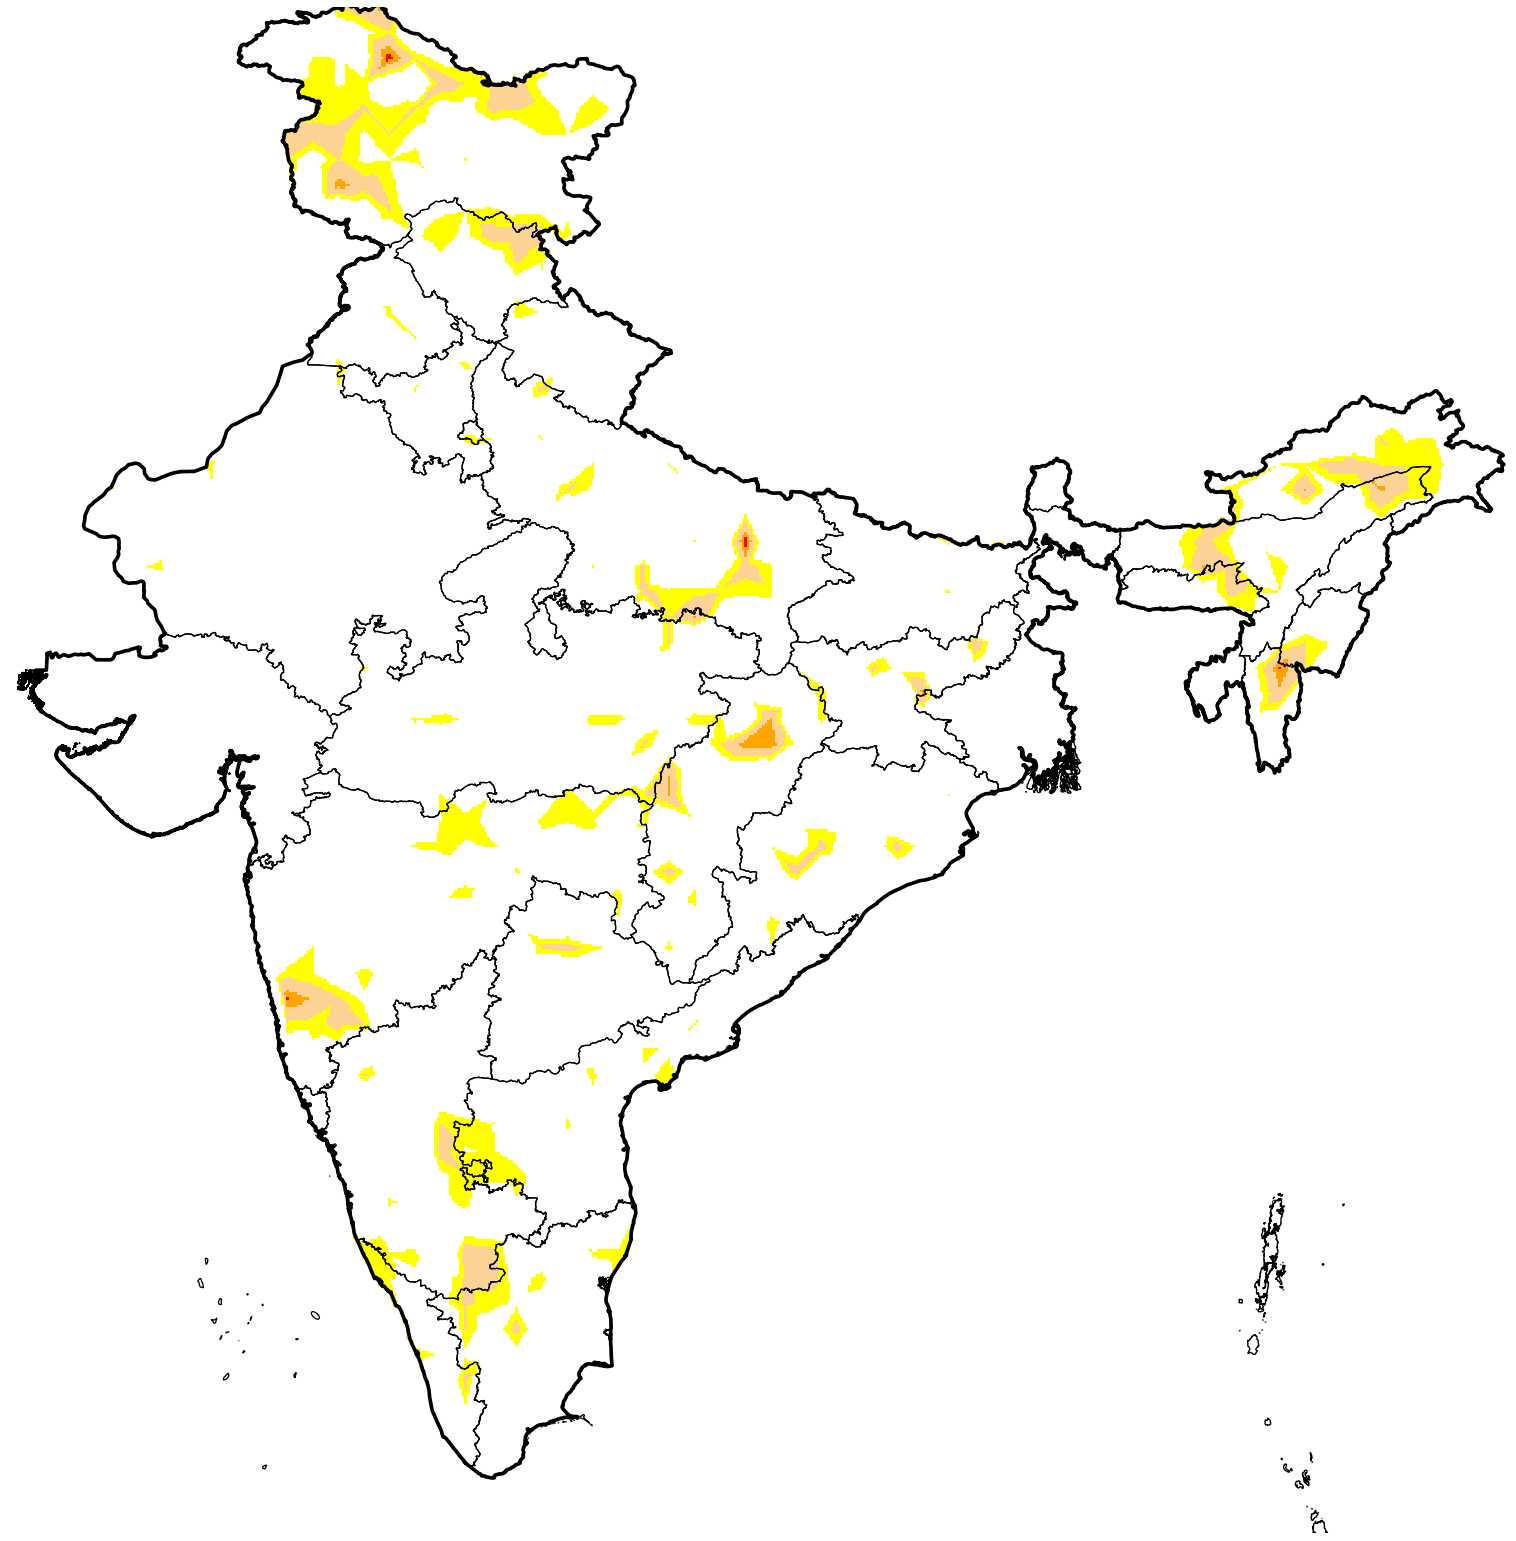
\includegraphics[width=0.60\textwidth]{cdi_map.png}\\[3pt]
  {\small\color{muted}{\latinfont Combined Drought Index (CDI) for the week ending May 20, 2026}.}
\end{center}
\vspace{2pt}
{\large\bfseries\color{titleblue}{\latinfont Summary}}\\[3pt]
{\justifying\normalsize\color{textblack}इदस्य सप्ताहस्य राष्ट्रिय-शुष्कता-परिस्थितिः प्रदर्शयति यत् भारतस्य बहुभागः अभी अपि सामान्य-श्रेणीयां तिष्ठति, यत्र {\latinfont 84.7} प्रतिशतं क्षेत्रं सामान्यरूपेण वर्गीकृतम् अस्ति। अस्मिन् सप्ताहे कुलक्षेत्रे शुष्कता-परिस्थितीः, विशेषतः डी० ({\latinfont D0)} इत्यने उच्चे, {\latinfont 15.3} प्रतिशतं क्षेत्रम् अनुभवात्। इदं संख्या पूर्ववर्तीकालेभ्यः शुष्कताक्षेत्रस्य संकुचनं प्रतिध्वनति, यतः कुलशुष्कताक्षेत्रम् सप्ताह-प्रति-सप्ताह {\latinfont 0.9} प्रतिशतबिन्दुः न्यूनम् भूत्वा, गतसप्ताहे {\latinfont 16.2} प्रतिशतात् अधुना {\latinfont 15.3} प्रतिशतम्। शुष्कतायाः सर्वाधिके प्रभावितानि प्रदेशानि दिल्ली-क्षेत्रम् अस्ति यस्य {\latinfont 52.2} प्रतिशतं क्षेत्रम् शुष्कतायां अस्ति, ततः मणिपुरः {\latinfont 42.3} प्रतिशतेन, मिजोरामः {\latinfont 40.8} प्रतिशतेन, अरुणाचलप्रदेशः {\latinfont 40.3} प्रतिशतेन, जम्मू-कश्मीरः {\latinfont 38.9} प्रतिशतेन, तथा मेघालयः {\latinfont 34.1} प्रतिशतेन अनुगच्छन्ति। विपरीता, पश्चिमबंगालः स्वक्षेत्रस्य {\latinfont 0.0} प्रतिशतं शुष्कतायां प्रति {\latinfont REPORT}ा, यदा राजस्थानम् शुष्कतायाः न्यूनतया प्रभावितराज्यम् अस्ति यस्य क्षेत्रस्य {\latinfont 1.0} प्रतिशतं शुष्कतायां अस्ति।\par}
\vspace{8pt}
{\large\bfseries\color{titleblue}{\latinfont Regional Outlook}}\\[2pt]
{\normalsize\color{titleblue}\textbf{{\latinfont North}}}\enspace {\normalsize\color{textblack}{\latinfont Moderate, scattered drought. About 28}\% {\latinfont of the area is in drought (D0}–{\latinfont D4)}.} \par\smallskip {\normalsize\color{titleblue}\textbf{{\latinfont Northwest}}}\enspace {\normalsize\color{textblack}{\latinfont Largely normal conditions. About 4}\% {\latinfont of the area is in drought (D0}–{\latinfont D4)}.} \par\smallskip {\normalsize\color{titleblue}\textbf{{\latinfont Northeast}}}\enspace {\normalsize\color{textblack}{\latinfont Moderate, scattered drought. About 27}\% {\latinfont of the area is in drought (D0}–{\latinfont D4). Pockets of severe-or-worse conditions are present}.} \par\smallskip {\normalsize\color{titleblue}\textbf{{\latinfont East}}}\enspace {\normalsize\color{textblack}{\latinfont Mostly normal, with localised dryness. About 7}\% {\latinfont of the area is in drought (D0}–{\latinfont D4)}.} \par\smallskip {\normalsize\color{titleblue}\textbf{{\latinfont Central}}}\enspace {\normalsize\color{textblack}{\latinfont Mostly normal, with localised dryness. About 15}\% {\latinfont of the area is in drought (D0}–{\latinfont D4). Pockets of severe-or-worse conditions are present}.} \par\smallskip {\normalsize\color{titleblue}\textbf{{\latinfont West}}}\enspace {\normalsize\color{textblack}{\latinfont Moderate, scattered drought. About 22}\% {\latinfont of the area is in drought (D0}–{\latinfont D4)}.} \par\smallskip {\normalsize\color{titleblue}\textbf{{\latinfont South}}}\enspace {\normalsize\color{textblack}{\latinfont Mostly normal, with localised dryness. About 16}\% {\latinfont of the area is in drought (D0}–{\latinfont D4)}.}
\end{document}
